\chapter{Metaheuristics}
Metaheuristics are high-level, problem-independent algorithmic that perturb the solution by moving it away from the current local optimum and attempting to get as close as possible to the global optimum. These algorithms can address various types of optimization problems with minimal adaptation. Even with a basic adaptation to a specific problem, they can often yield good solutions for certain instances. Specifically for the TSP, metaheuristics can typically find better solutions than any 2-opt variation within a reasonable time limit. These techniques essentially allow for the exploration of the solution space, avoiding stagnation in local minima or maxima with objective function values that are far from the global optimum.

In the following sections, we will present two different metaheuristic algorithms:
\begin{itemize}
    \item \textbf{Tabu Search}: When a local minimum is reached adds certain edges to a tabu list, making them forbidden for an improving move. And force the exploration of new situations.
    \item \textbf{Variable Neighborhood Search (VNS)}: Randomly alters \( k \) different edges from the current solution and improves it using 2-opt.
    %\item \textbf{Genetic Algorithm}: Simulates Darwin's theory of evolution, aiming to generate the %fittest population, which may contain a good solution.
\end{itemize}

\section{Tabu Search}
\label{chap:tabusec}
Designed by Fred W. Glover \cite{tabusearch}, the Tabu Search algorithm allows for modifying a given local optimum solution, even at the cost of worsening it, with the goal of exploring the solution space more thoroughly. At each iteration of the algorithm, the solution is modified with a new tour belonging to its 2-opt neighborhood.

To prevent these modifications from leading to the exploration of already visited local minima, a list of ''forbidden moves'' is created, called \(Tabu\) \(List\), which is a FIFO (First In First Out) queue with a specific size. The size of the tabu list is referred to as \(tenure\). This way, a move won’t remain illegal forever but just for a certain number of iterations. 

The performance of this algorithm can depend on the tenure of the list. If it is too small, the algorithm gets stuck in the local minimum because there is a sequence of moves that brings the solution back to the local minimum. Conversely, if the tenure is too large, the search is not effective because the neighborhood is too small.To overcome this, there are some options to dynamically adjust the tenure during execution.\\

There are many different policies to change the Tabu tenure dynamically. The policies considered in this case were:
\begin{itemize}
    \item \textbf{Step policy}: Changes the Tabu List size every \(K\) iterations to a minimum or a maximum.
    \item \textbf{Linear policy}: The Tabu List size grows by 1 unit for each iteration until reaching the maximum size, then decreases by 1 unit for each iteration until reaching the minimum size, and so on.
    \item \textbf{Random policy}: Changes the Tabu List size every \(K\) iterations to a random size chosen within a range.
    \item \textbf{Reactive policy}: The maximum tenure is equal to \(1/K\) (with \(K\) arbitrary) of the number of nodes of the instance to be solved, while the minimum is equal to half of this value.
    \item \textbf{Static policy}: The value of the tenure does not change during the execution.
\end{itemize}

The variant implemented in the code is the \(Static\) \(Policy\), that is the simplest one. A dynamic policy may create better results in theory, but it also requires more computation time. In average, with our input sizes, it should make almost no difference, so we went for the simplest solution.\\

When, during the execution, the method encounters an edge that is tabu, it skips that edge. This ensures that other solutions are explored rather than reverting to the previous ones. When the best non-tabu couple of edges is found, the algorithm does a 2-opt step. It may happen that the best non-tabu swap is a worsening 2-opt move, it would mean that the algorithm reached a local minimum and it is trying to escape from it. 
When the tabu list is full and the method needs to add a new node, the oldest one is removed to make space.
The termination criterion for the algorithm can be defined by either the expiration of the available time or the achievement of a maximum number of iterations. In our code, we used the time-based criterion. The solution provided by the algorithm is the best one identified up to the point of termination.

\newpage

\noindent The Tabu Search pseudocode is shown in Algorithm~\ref{alg:tabu_algo}.

\begin{algorithm}
    \caption{Tabu Search}
    \label{alg:tabu_algo}
     \begin{spacing}{1.2} % Adjust this value to change line spacing
        \KwIn{TSP Istance with a feasible solution}
        \KwOut{A valid tour}
        \BlankLine
        result $\leftarrow$ best solution found so far\;
        cost $\leftarrow$ cost of result\;
        tenure $\leftarrow \max(\text{inst.nnodes} / 10, 10)$\;
        \BlankLine
        \While{time elapsed $<$ time\_limit}
        {
            \ForEach{node pair (A, B)}
            {
                \textbf{if} \textit{A or B in TabuList} \textbf{then Skip}\;

                \BlankLine
                compute \KwSty{swap} costs\;
                \If{fist iteration \textbf{or} new cost $<$ bestCost}
                {
                    bestSol $\leftarrow$ updated solution\;
                    bestCost $\leftarrow$ new cost\;
                    swappedNode $\leftarrow$ node A\;
                }
            }
            \BlankLine
            \If{bestCost $\geq$ cost}
            {
                \KwSty{add} swappedNode \KwTo tabu list\;
            }
            \BlankLine
            result $\leftarrow$ bestSol\;
            cost $\leftarrow$ bestCost\;
        }
    \end{spacing}
\end{algorithm}

\section{Variable Neighborhood Search (VNS)}
The Variable Neighborhood Search (VNS) algorithm, introduced by N. Mladenović and P. Hansen \cite{MLADENOVIC19971097}, aims to enhance a given local optimum by starting with an arbitrary solution and exploring neighborhoods of different sizes, as illustrated in Figure~\ref{fig:vns}. 
The idea of the VNS algorithm is that Tabu Search waste too much time to escape from a local minimum. 

\newpage

\noindent That time should instead be used for optimization. That is why it uses a quick way of escaping: the kick. This method is also a less controllable way that does not assure good results since it may fall back to the same local minimum.
VNS is founded on three key principles:

\begin{itemize}
    \item A local minimum in one neighborhood structure may not be the same in another.
    \item A global minimum is a local minimum in all neighborhood structures.
    \item Often, a local minimum in one neighborhood structure is near a local minimum in another.
\end{itemize}

\begin{figure}[H]
    \centering
    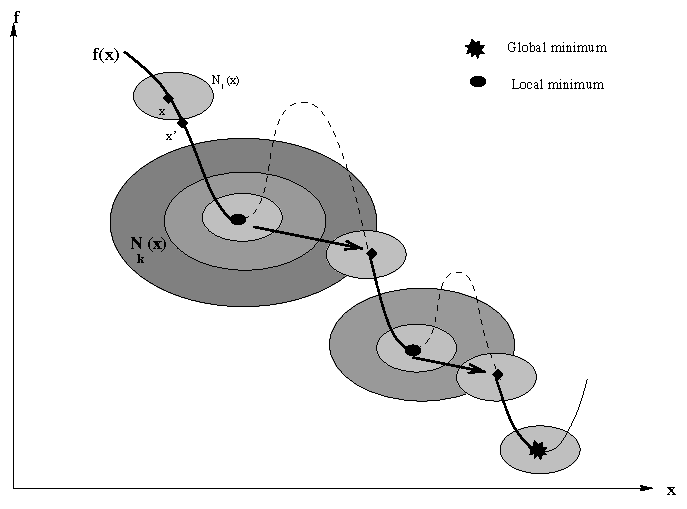
\includegraphics[width=0.65\linewidth]{Immagini/vns.pdf}
    \caption{An illustration of the Variable Neighborhood Search (VNS) process \cite{Hansenvns}.}
    \label{fig:vns}
\end{figure}

If a superior solution is not discovered in the neighborhoods of size \( K \), the algorithm randomly selects and replaces certain branches with other edges \cite{Hansen2019}. This introduces a temporary increase in cost, with the expectation that a new neighborhood will lead to a solution that diverges from the initial local optimum.

VNS repeatedly refines the current solution until a local minimum is achieved (intensification phase), using the 2-opt method. Subsequently, the algorithm picks a random solution within the neighborhood (diversification phase) as shown in the Figure~\ref{fig:vns_kick}. If this new solution is better than the best one found so far, it becomes the new best solution. In the next iteration, the algorithm starts with the smallest neighborhood; if no improvement is found, it moves to a larger neighborhood.

\begin{figure}[H]
    \centering
    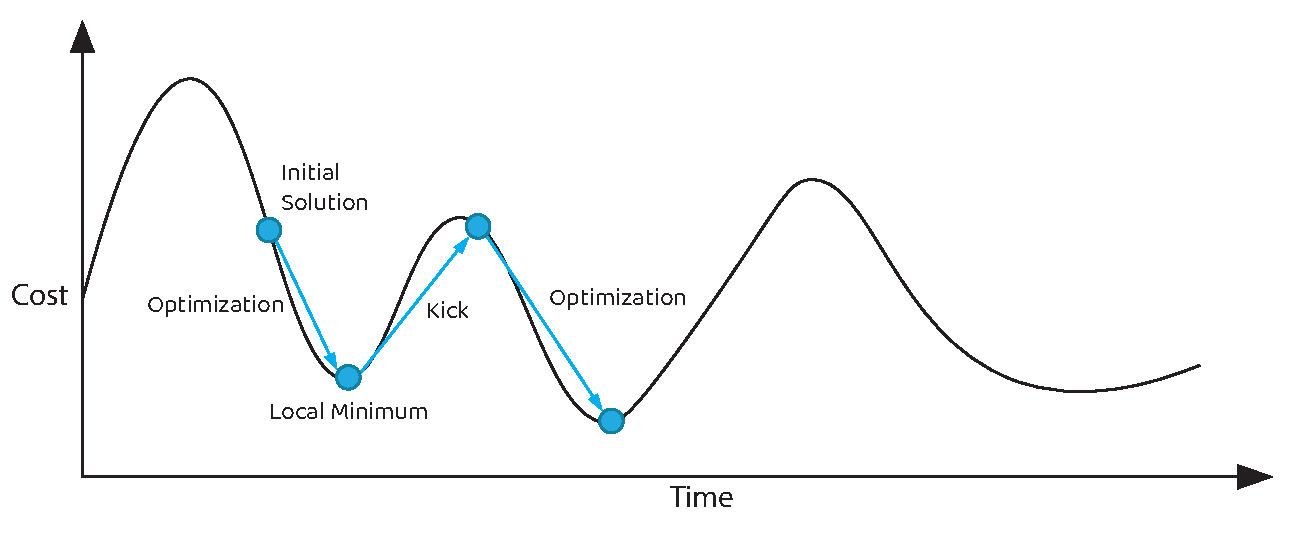
\includegraphics[width=0.85\linewidth]{Immagini/vns-kick.pdf}
    \caption{An illustration of the Variable Neighborhood Search (VNS) process.}
    \label{fig:vns_kick}
\end{figure}

The algorithm \ref{alg:vns_algo} concludes when a user-defined time limit is reached or after a set number of iterations, returning the best solution found. This method retains much of the initial solution, preventing the loss of previously gathered information.

\begin{algorithm}[H]
    \caption{Variable Neighborhood Search}
    \label{alg:vns_algo}
    \begin{spacing}{1.2} % Adjust this value to change line spacing
        \KwIn{TSP instance}
        \KwOut{A valid tour}
        \BlankLine
        Initialize result vector with best solution found so far\;
        \While{time < time\_limit}
        {
            performTwoOptOptimization()\;
            \For{$i \leftarrow 1$ \KwTo random number between 2 and 10}
            {
                applyKick()\;
            }
        }
        \BlankLine
    \end{spacing}
\end{algorithm}

The implementation presented here considers only the 3-opt neighborhood. This means that during the kick operation \ref{alg:kick_func}, three edges are randomly removed and reconnected in a predefined manner.

\begin{algorithm}[H]
    \caption{Kick Function \textit{applyKick()}}
    \label{alg:kick_func}
    \begin{spacing}{1.2} % Adjust this value to change line spacing
        \KwIn{Solution vector, cost}
        \KwOut{Updated solution vector and cost}
        Randomly select indices $i$, $j$, $k$\;
        Update the solution vector by swapping sub-sections between $i$ and $j$ and between $j$ and $k$\;
        Adjust the cost based on the new configuration\;
        \BlankLine
    \end{spacing}
\end{algorithm}

\section{Comparison between Metaheuristics}
We have seen two important metaheuristic algorithms applied to the TSP. Here we compare the two algorithms in terms of costs of the solution found.

Figure \ref{fig:tabu_vns} illustrates the cost comparison between our implementation of the Tabu Search algorithm and the Variable Neighborhood Search (VNS) algorithm. Both were given a time limit of 60 seconds.

As we can see they gave mostly the same results. The ability of VNS to outperform Tabu Search in some cases suggests that it can offer advantages in certain situations, though not consistently. Similarly, the inferior performance of VNS in other cases indicates that Tabu Search maintains a competitive robustness. Overall, this analysis confirms the qualitative equivalence of the two implementations in our application context.

\begin{figure}[H]
    \centering
    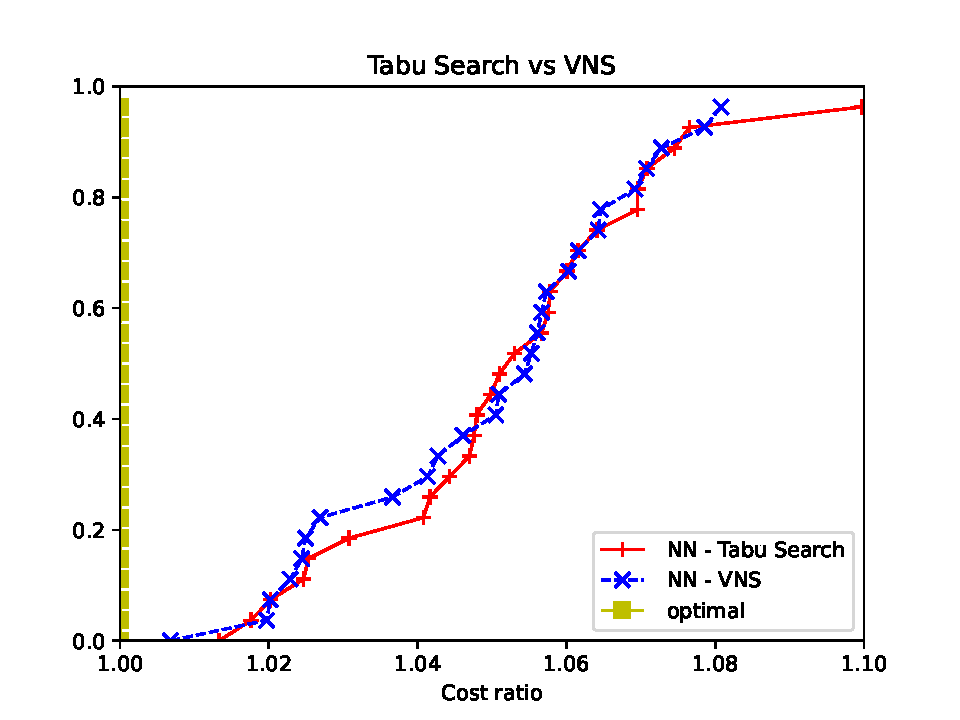
\includegraphics[width=0.7\linewidth]{Immagini/Tabu vs VNS.pdf}
    \caption{Performance Profile of Tabu Search and VNS.}
    \label{fig:tabu_vns}
\end{figure}
